\documentclass{article}
\usepackage{graphicx}
\usepackage{amssymb}
\usepackage{amsmath}
\usepackage{float}
\usepackage{hyperref}
\usepackage[margin=1in]{geometry}

\begin{document}

\title{Robotics 811 - Homework 4}
\author{Xiang Zhi Tan}
\maketitle

\section{Q1}
\section{Q2}
\subsection*{2(a)}
Firstly, we plotted the function in matlab using the \textit{contour} function on the range, $y=[-4,2]$ and $x=[-2,4]$. Following is the result of the contour plot
\begin{figure}[H]
\centering
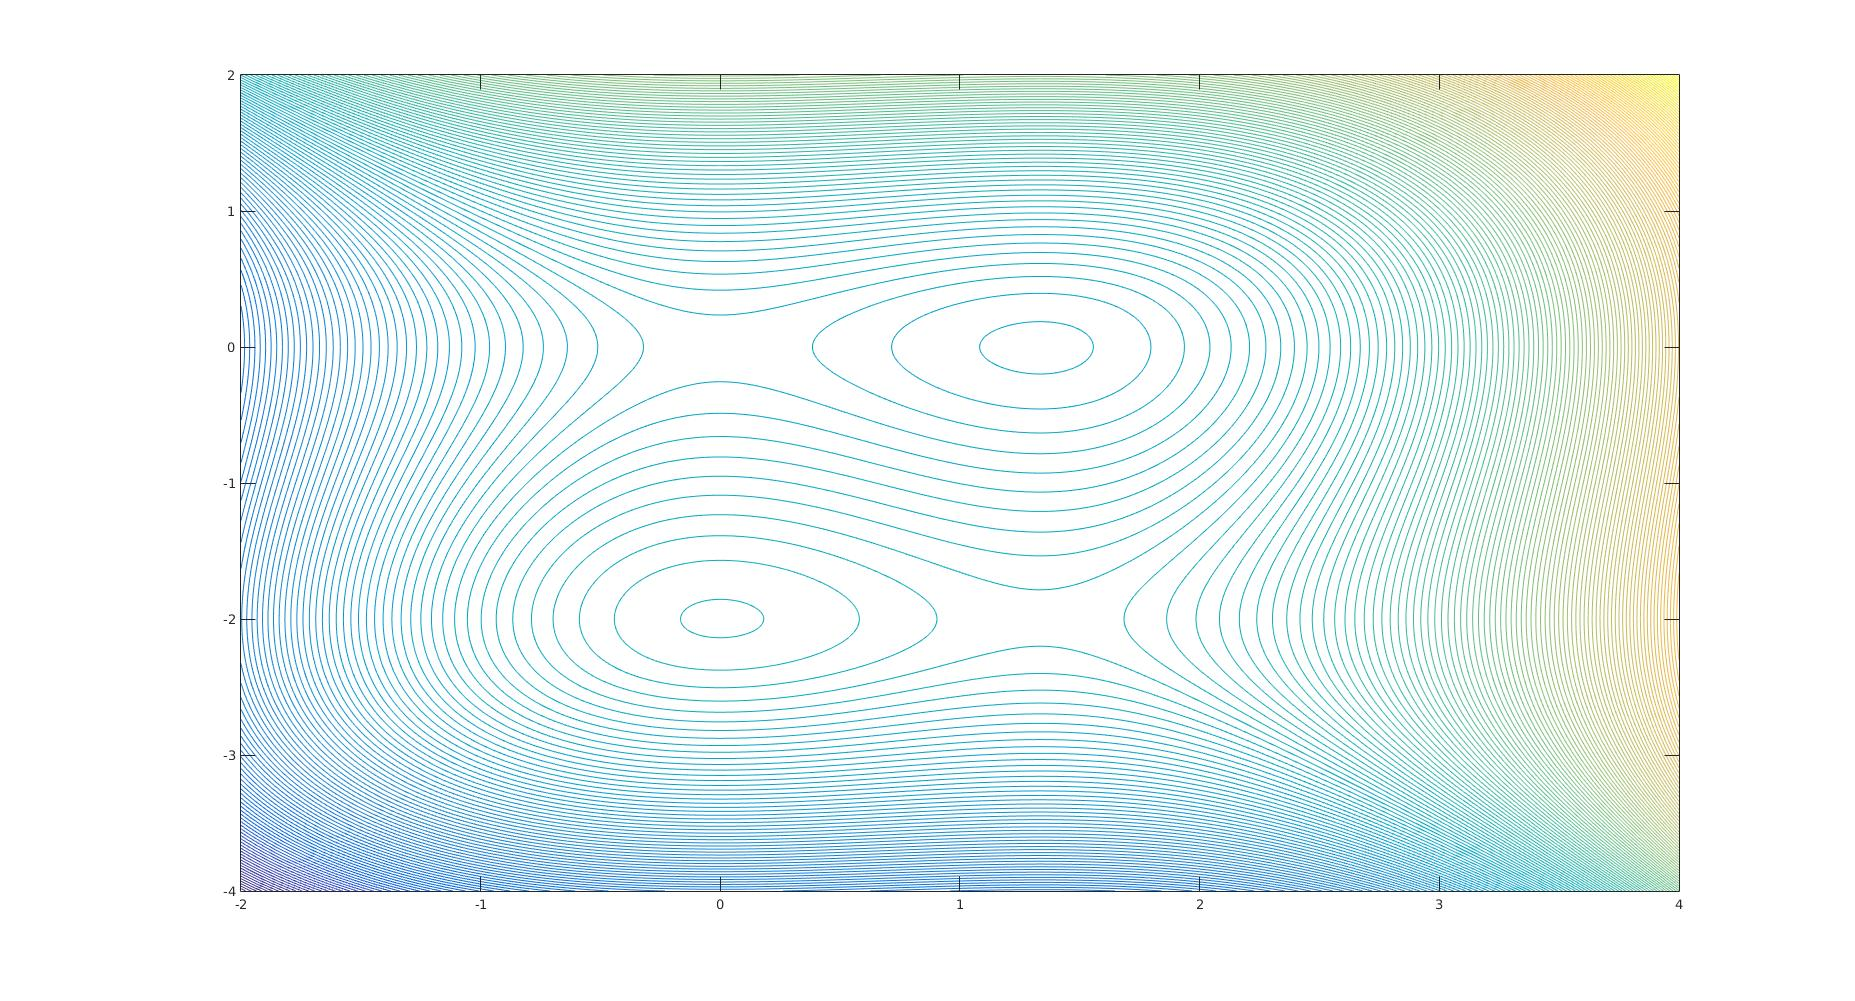
\includegraphics[width=6.5in]{figures/2a.jpg}
\caption{plot of the function $f(x,y) = x^3 + y^3 -2x^2 + 3y^2 - 8$}
\end{figure}
By examining the sketch created, we notice there are four critical points, $(0,-2),(0,0),(\frac{4}{3},-2),(\frac{4}{3},0)$.
We then measure the gradients(in the domain space) of the nearby points to determine the type of critical point. 
Following are the finding for each point:
\begin{enumerate}
\item Point$(0,-2)$\\
This is a local maxima. By measuring the gradient at 8 points around the point with a step size of $0.1$ relative to this point. we found them all to have a position gradient which means they are moving upwards towards $(0,-2)$ which means this is a local maximum\\
\item Point$(0,0)$\\
This is a saddle points. When measuring the gradient at 8 points around the point with a step size of $0.1$ relative to this point, we measured a positive gradient at the two points of $(0.1,0)$ and $(-0.1,0)$ to have a negative gradient where as the remaining 6 points to have a negative gradient. This fits the definition of a saddle point.
\item Point$(\frac{4}{3},0)$\\
This is the local minima. When measuring the gradient at the 8 points around the point with the step size of $0.1$ relative to this point, all gradients are negative, this means that the direction of all these points are towards this point meaning that this point must serve as the local minima.
\item Point$(\frac{4}{3},-2)$\\
This is a saddle points. When measuring the gradient, we found a negative gradient at point $(1.23333,-2)$ and $(1.43333,-2)$ and positive gradient at all remaining points. This shows that this must be a saddle point.
\subsection*{2(b)}
The gradient(partial derivative) of x and y can be found with the following equation:
\begin{equation*}
\begin{aligned}
\frac{\partial}{\partial x}  = x(3x - 4)\\
\frac{\partial}{\partial y}  = y(3y + 6)
\end{aligned}
\end{equation*}
Using the steepest descent algorithm, we first calculate the gradient at point $(1,-1)$. Which gives us the gradient at x, $\frac{\partial}{\partial x} = -1$ and gradient at y, $\frac{\partial}{\partial y} = -3$. Since the gradient are both non zero, we try to minimize the function $g(t) = f(x + t\vec{u})$ with u being the gradient. Minimizing the function, we found $t = \frac{1}{3}$. We update the points using the following algorithm $x^{n+1} = x^{n} - t\vec{u}$. After updating the points, we found the points to be $(\frac{4}{3},0)$ which is one of the critical points(also the local minima). The gradient at that point is also $0$, stopping the algorithm. Therefore, we need only one step to converge to the local minimum.

\end{enumerate}

\section{Q3}
\section{Q4}
\section{Q5}
\section{Q6}
\section{Q7}
\end{document}